%!TEX root = ../Thesis.tex
\chapter{interpretTheForest}

\section{Modeling with random forest}
The random forest model started to play a bigger role for this thesis as it showed to outperform linear regularized regression models as partial least squares and elastic net. Also RF seem to outperform the non-linear k-nearest neighbor. The random forest algorithm is certainly not always the best choice of model, the non free lunch theorem states that the is not optimal silver bullet. That said Random forest together with radial suppert vector machine and gradient boosting was in comparison on 110 data sets found to be the in generel top performing algorithm in terms of cross-validated accuracy \cite{Citewainer2016comparison}. If the underlying model generating the data is truly linear, e.g. in octane concentration determination in near-infrared light spectroscopy \cite{kalivas1997two}.


\section{One interpretation of interactions}
Throughout the work of this thesis, there have been an emphasis on identifying and visualizing interactions. In this process, I have made my own working definitions of interactions, that especially relate to geometrical interpretations of model structures. In our paper \textit{Forest Floor Visualizations of Random Forests} we introduce an interaction as:

\begin{quotation}
\textit{
"Interactions in the model structure mean that the model predictions in part rely on the interplay on two or more features. Thus, the interaction parts of a model structure cannot be reduced to additive scoring rules, one for each feature. Likewise, to plot single feature-to-prediction relationships is not a sufficient context for visualizing any interactions."
}
\cite{welling2016forest}
\end{quotation}

To discuss this definition of interactions in model structures, below is given a definition of model structures, feature spaces and predictions spaces. A given model structure $f$ maps from feature space $X$ to a prediction space $\hat{y}$, such that $\hat{y} = f(X)$. $X$ is a real valued euclidean vector space, constituted by $d$ axes $x_1$,...,$x_d$. Any point is a unique combination of feature values.
\footnote{See the forestFloor article \cite{welling2016forest} or this how to handle categorical features, an idea originally from Friedmans gradient boosting and partial dependence article \cite{friedman2001greedy}.}
For regression the prediction space $\hat{y}$ is simply an one-dimensional real axis. We understand $f$ as a function which connect any point in the feature space to some point in prediction space. To discuss how to describe interactions, I will introduce a simple analogy structure. We can imagine the surface of the regression function $f$ in a Eucledian 3D space, for two features $x_1$ and $x_2$ spanning the horizontal plane and one vertical prediction axis. We call this joint feature space and prediction space for the mapping space. We can imagine the structure of $f$ is a geographical landscape model of altitude as function of coordinates. This $f$ map has potentially valleys and mountains. Essentially, if $f$ can be reduced into separate additive score functions, we can for any ($x_1$,$x_2$) coordinate position in this landscape not only use $f$ to calculate the altitude, but also $f$ decomposed into $f_1$ and $f_2$, such that $\hat{y} = f(X) = f_1(x_1) + f_2(x_2)$. When the mapping space is only 3D, it is not obvious, why we want to decompose $f$. However, for higher dimensional models, we cannot directly visualize nor comprehend the geometrical structure. By decomposing the model structure we allow ourselves to split the full structure in to simpler pieces we can visualize and understand. Unfortunately not all landscapes can be reduced to such additive scoring rules. Returning to the altitude model $f$, imagine a landscape model of a single pyramid surrounded by a flat dessert, see Figure \ref{pyramid}. A function describing the local height of this landscape would reflect, that only when $x_1$ AND $x_2$ match the position of the pyramid, the predicted altitude should rise above the sands. To decompose this topological map into $f_1$ + $f_2$ would analogously correspond to two observers on either side of the pyramid. Neither can see the entire pyramid but only their respective front sides. Either observer would notice that in the middle of their respective fields of view, the altitude is elevated due to the pyramid. Each observer could generalize what they see to a partial function parallel to their field of view. However, as they cannot see their back side of the pyramid, neither of the observers will know if this is generally true for any position on the other axis. If we simply combined by averaging the altitude predictions of the two naive observers, the model structure would more look like the roof of a tower, not a pyramid. 

\begin{figure}
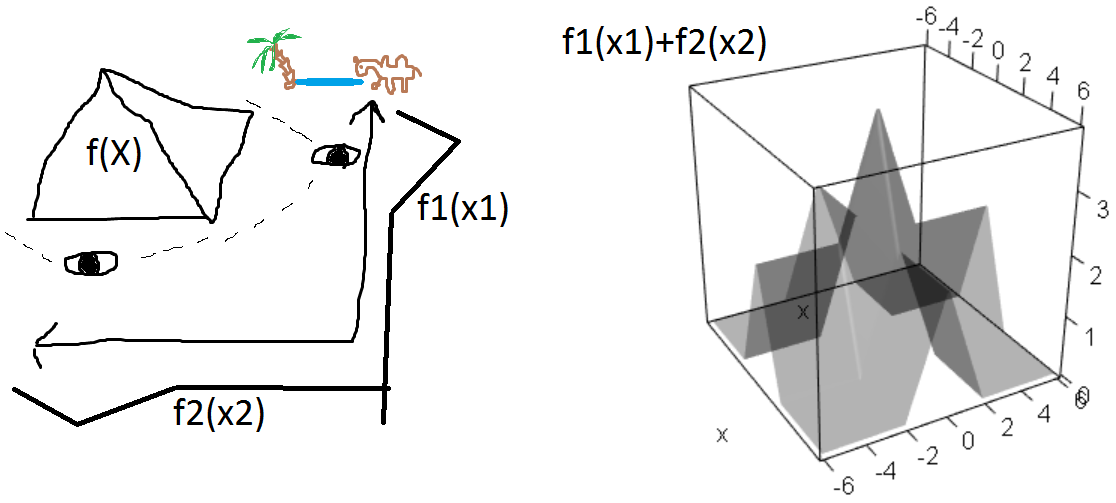
\includegraphics{graphics/sketch_pyramid_interaction.png}
\caption{Pyramid in flat sands, an example of a model structure with non-global non-saddle interaction.}
\label{pyramid}
\end{figure}

In the mini review (letter) of boulesteix \textit{et al} points out that the definition of interations can be vague and ambiguous in recent litterature \cite{boulesteix2014letter}. They refer to the simple classical statistical logit-model, that contains a two-variable saddle point interaction. Here $f$ is decomposed such that $\hat{y} = f(X) = P(\beta_1 x_1 + \beta_2 x_2 + \beta_{12} x_1 x_2)$ where $P$ is the logit transfer function $P(z) = log(\frac{z}{1-z})$. The logit function is used to let $\hat{y}$ describe the probability of some binary outcome. We can generalize and say $P$ can be any polynomial function. To include an interaction term in a model structure as the product of two variables is called a saddle point structure. Even when the product of two variables is wrapped in a transfer function $P$, this interaction is a saddle point. The transfer function $P$ can be seen as a compression/rearrangement of the $\hat{y}$ prediction axis. The limitation of the saddle point structure is that it can neither fit shape of the pyramid, because the pyramid is a local interaction in an otherwise flat dessert sand landscape with no interaction structures. My postulate is that there is no combination of compressing, stretching and loop of the $\hat{y}$ axis, which can morph a saddle point structure into the pyramid structure. Therefore I argue that logistic models comprised by the coefficient weighted sum of main effects and a number of saddle point interactions and a transfer function $P$ is not a suitable basis for decomposing any model structure as there are structures which do not fit this scheme. Or put in a for any $f_12$ there is not necessarily a $P$ such that $f_{12}(x_1,x_2) = P(\beta x_1+ \beta x_2 + \beta_{12} x_1 x_2$. 

((Insert proof by contradiction))

To fit the structure of the pyramid within classical statistics, one would probably resort to splines \cite{harrell2015regression}.

To decompose any possible landscape, including the pyramid, let 
$f(X)= f_1(x_1) + f_2(x_2) + f_12(x_1,x_2)$. If $f_{12} = f$ then not much have been accomplished. In fact their are a lot of really unuseful decompositions of $f$. In general it would be helpful to describe as much of the structure as possible as additive main effects and only what absolutely cannot be described as a higher order interaction. Let us imagine the pyramid is placed in a landscape steadily descending towards a ocean. Then the lower $f_1$ and/or $f_2$ can describe this general trend, while $f_12$ describe the pyramid.

A non-linear regression model of $d$ features can be decomposed into bias/offset, $d$ main effects, $d-1$ second order effects, $d-2$ third order effects, and so on until $1$ $d^{th}$ order effect. The type of decomposition we aim for is one which explains as much of the structural features in lowest order effects. In the following I calculate the number of possible components approximately doubles per feature.

For a model of $d$ features there will be effects of $d$ different orders. The smallest of first order (main effect) and the highest of $d$ order. The number of combinations to draw $i$ features in a $d$-features can be described as binomials. Summing all binomial counts from $i=1$ to $d$ give the number possible components/effects of the system. Therefore, $n_d$ the number of possible effects is calculated as
$n_d = \sum_{i=1}^{d} \binom{i}{d}$. Furthermore the number $n_d$ can be defined by $n_{d-1}$ as,
$n_d = 2n_{d-1} + d$. For $d=10$ there are staggering $2036$ possible components effects. Suddenly one may get sweaty hands, when learn there are so many different effects of a multivariate model with 10 features. The promise that decomposition of the model would bring simplicity and clarity seem far from for filled. Fortunately we can ignore a high number of these components when emphasising model structures trained by random forest or any other reasonable machine learning algorithm. As shown in supplementary materials for the forest floor article, random forest can only poorly fit an saddle point interaction of 3 orders and 4 orders is nearly impossible. We live in a reality where fifth order interactions always will be near impossible to robustly estimate with statistical models and finitely sized training sets. Adhering to the Occam's Razor guideline, that we should always pick the simplest model explaining the observed data, it is very unlikely there would not be a second, third or fourth order interaction which could explain the same observations. Therefore can all effects of more than 2 or 3 orders be disregarded. Furthermore, a subset of features will often be used more frequently than others in splits in the trees of the random forest. Interactions terms only can be learned in a tree model when one split by one feature is conditioned by another feature split upstream. As the most dominant features tend be the ones upstream, interactions in the model structure are most likely found in the model structure as second order interactions between one relatively dominant feature (high variable importance) and another feature. Therefore can interactions between weak features be disregarded at first. Therefore can a random forest model be decomposed into $d$ main effects and a lower number of second order effects. Where one or both both features tend have been a favorite splitting feature. To summarize, an interaction effect of $i^th$ order is one, that cannot be fully be described by any combination of lower order effects.

This broad definition of interaction effects can also cover classification and multi classification, where $f$ map to a $K-1$ dimensional simplex probability space, where $K$ is the number of classes. Second order interaction effects for a probabilitic classification model mapping to 3 classes($K=3$) are visualized in the forest floor article, see figure 12 \cite{welling2016forest}. However, the surface of this second order interaction effect is not 2 dimensional as the pyramid example. For a second order interactions($i=2$), the mapping space has $i+K-1=2+3-1=4$ dimensions. In the forest floor article a such 4D problem is visualized in Figure 12. Here a 2D triangular (K-1)-simplex diagram is used to describe the probability distribution of predictions, and different color gradients in turn represent the different feature axes. 
\footnote{If number of classes $K>=5$ is higher than 5, the (K-1)-simplex diagram would require a 4D or higher visualization. Instead Figure 10 of article depicts how to plot probability predictions by each class by a single axis.}

Returning to pyramid example. Let's say $f_1$ described the gradual descending of the landscape towards the ocean. As $f_1$ is non-linear, it could describe a single sand dune, a local maximum, at the beginning of the beach. This local sand dune will now stretch infinitely to both sides, such that for any $x_2$ the effect of $f_1$ is static. We can use this observation make a bottom up definition of interactions also. Let $S$ be a subset of all features $X$ of the model. Let $T$ bet the complimentary subset of features $S \\ X = T$. An interaction effect by a subset $S$, $f_S$, has the order equal to size of $|S|$. We would now that $f_S$ is a useful decomposition of $f$, as for every parallel plane spanned by the features the curvature are the same. In contrary when the  interaction curvature is far from the same any combination of feature vales of $T$, we know we're missing an important higher order interaction. Furthermore the the feature axis of which the $S$-plane curvature changes the most is the one feature from $T$ which need to be indluded in $S$ in order to obtain suitable generelized effect that is static for any point in the $T$-plane.


For a model structure with a a predicted response $\hat{y}$ 

The decision tree ensemble random forest have a series of useful diagnostics which have been used in this thesis work.

\section{Other ways to identify interactions}

2-way partial dependence plot

minimal subtree \cite{ishwaran2010high}



\section{Article: Forest Floor Visualizations of Random Forests}

First version submitted to arXiv.org the 30$^{th}$ of May 2016.
Latest version (3$^{rd}$) submitted to arXiv.org the 4$^{th}$ of Luly 2016

\newpage
\includepdf[pages={1-},scale=0.90,pagecommand={\pagestyle{myruled}}]{chapters/forestFloorArt.pdf}

\includepdf[pages={2-},scale=0.90,pagecommand={\pagestyle{myruled}}]{chapters/supplementaryForestFloor.pdf}